%% BloomBot: IEEE conference-format project report
%% Authors: C. Murali Madhav, Amathziah J, Ravi Yadav, Pugazhendhi J
%% Affiliation: Newton School of Technology, Rishihood University, Sonipat, India
%% Build: cd docs/report && tectonic bloombot_ieee.tex
%% Every number comes from docs/RESULTS.md and results/ in this repository.

\documentclass[conference]{IEEEtran}
\IEEEoverridecommandlockouts

\usepackage{cite}
\usepackage{fontspec}
\setmainfont{texgyretermes}[Extension=.otf, UprightFont=*-regular, BoldFont=*-bold, ItalicFont=*-italic, BoldItalicFont=*-bolditalic]
\usepackage{amsmath,amssymb,amsfonts}
\usepackage{graphicx}
\usepackage{textcomp}
\usepackage{xcolor}
\usepackage{booktabs}
\usepackage{multirow}
\usepackage[hidelinks]{hyperref}
\usepackage{url}
\usepackage{tikz}
\usetikzlibrary{positioning,arrows.meta,fit,backgrounds,calc}

\setlength{\textfloatsep}{6pt plus 2pt minus 2pt}
\setlength{\floatsep}{6pt plus 2pt minus 2pt}
\setlength{\intextsep}{6pt plus 2pt minus 2pt}
\setlength{\abovecaptionskip}{3pt}
\setlength{\belowcaptionskip}{0pt}
\setlength{\dbltextfloatsep}{6pt plus 2pt minus 2pt}
\renewcommand{\arraystretch}{1.0}

\definecolor{lexblue}{RGB}{25,79,129}
\definecolor{llmamber}{RGB}{176,97,31}
\definecolor{checkgreen}{RGB}{16,108,62}
\definecolor{softgrey}{RGB}{95,99,108}
\definecolor{fillblue}{RGB}{215,234,255}
\definecolor{fillamber}{RGB}{252,236,214}
\definecolor{fillgreen}{RGB}{220,240,226}
\definecolor{fillgrey}{RGB}{240,238,233}

\newcommand{\best}[1]{\textbf{#1}}

\begin{document}

\title{BloomBot: Bloom-Level Classification of Exam Questions Across Institutions, and Rebalancing of Question Papers with Verified Rewrites}

\author{%
\IEEEauthorblockN{C.~Murali Madhav,\; Amathziah J,\; Ravi Yadav,\; Pugazhendhi J}
\IEEEauthorblockA{Newton School of Technology, Rishihood University, Sonipat, India}}

\maketitle

\begin{abstract}
Outcome-based education asks teachers to tag every exam question with a level of the revised
Bloom taxonomy and to keep a paper's mix of levels within a blueprint. Published automatic
classifiers report 0.73--0.94 accuracy, but only when trained and tested on the same dataset.
On 9,855 questions from seven sources we reproduce the cross-dataset drop (0.32 weighted F1 for
TF-IDF with an SVM) and trace much of it to \emph{concept shift}: institutions label the same
wording differently (``Explain\,\ldots'' is Understand in 93\% of one Malaysian set but
Remember in 55\% of Indian engineering questions). BloomBot answers this with three design
choices. It parses the \emph{directive} a question gives instead of matching any Bloom verb;
it trains an ordinal classifier on delexicalised linguistic features and a small sentence
embedding with sources balanced; and it lets a college adapt the model with a few labelled
questions. Trained on all other sources, it reaches 0.641 weighted F1 on an unseen source,
+0.051 over TF-IDF with an SVM ($p<0.001$), and 0.630 on a never-trained-on Indian school-board
set, with 82\% of predictions within one level. Labelling 100 of a college's questions adds
0.07 on average. A 4-billion-parameter open LLM is worse than this CPU model on its own, badly
calibrated and sycophantic, but as a reasoning second opinion on uncertain questions it adds
+0.042 weighted F1 under nested selection. To rebalance a paper, BloomBot plans the fewest
rewrites that meet the blueprint and accepts a rewrite only after an independent classifier,
form and topic checks and a ``could memory alone answer this?'' test; 37 of 40 rewrites pass.
The whole system runs on a laptop CPU.
\end{abstract}

\begin{IEEEkeywords}
Bloom's taxonomy, question classification, cross-dataset generalisation, concept shift,
ordinal regression, large language models, educational assessment
\end{IEEEkeywords}

% =============================================================================
\section{Introduction}

Colleges that follow outcome-based education (OBE) map each exam question to a cognitive level
of the revised Bloom taxonomy (Remember, Understand, Apply, Analyze, Evaluate, Create)
\cite{bloom1956,anderson2001} and are expected to keep lower-order questions in check. India's
AICTE \emph{Examination Reform Policy} gives, as an example, a cap of 40\% weightage on
knowledge-oriented questions \cite{aicte2018}. Tagging by hand is slow and inconsistent, and a
paper can satisfy the level mix while being impossible to finish in the time allowed.

Automatic Bloom classification has a long history, from SVMs on item banks \cite{yahya2012}
and taxonomy features \cite{sangodiah2017} to modified TF-IDF with word2vec \cite{mohammed2020}
and CNNs over pre-trained embeddings \cite{gani2023}. Most report accuracy on random splits of a
single dataset. A teacher at a new college faces a different problem: the classifier was
trained on someone else's questions. Faraji \emph{et al.} \cite{faraji2026} measured this
directly and found an average drop of about 0.25 F1 when a model is tested on another dataset.

This report describes BloomBot, a system built around that gap. Our contributions are:
\begin{itemize}
\item A provenance-checked corpus of 9,855 questions from seven sources, with cross-source
  de-duplication and one source kept strictly for testing, and a reproduction of the
  cross-dataset drop (Section~\ref{sec:data}, \ref{sec:results}).
\item Evidence that much of the drop is \emph{concept shift} between institutions, which no single
  model can remove, and a k-shot institution profile that recovers 0.07--0.10 weighted F1 with
  100 labelled questions.
\item A CPU-only classifier that parses the directive of a question and is ordinal and
  source-balanced; it transfers better than TF-IDF and embedding baselines and resists verb traps.
\item A measured account of a small open LLM in this task: worse alone, overconfident and
  sycophantic, yet useful as a reasoning second opinion when combined by a linear mixture,
  and harmful when combined by the commonly used log-linear pooling.
\item An end-to-end paper checker: parsing of real papers, a level mix weighted by marks
  against a blueprint, a time and marking check, and a rewrite loop whose every output is
  verified by components other than the one that wrote it.
\end{itemize}

% =============================================================================
\section{Related Work}

\textbf{Bloom classification.} Yahya \emph{et al.} \cite{yahya2012} classified 600 item-bank
questions with an SVM. Sangodiah \emph{et al.} \cite{sangodiah2017} added taxonomy-based features;
Mohammed and Omar \cite{mohammed2020} weighted TF-IDF by part of speech (TFPOS-IDF) and combined it
with word2vec; Gani \emph{et al.} \cite{gani2023} used CNNs with pre-trained embeddings on Malaysian
university exams. Scaria \emph{et al.} \cite{scaria2024} generated questions at each level with LLMs
and had two experts label them, which gives a cleanly labelled but machine-written source.

\textbf{Cross-dataset evaluation.} Faraji \emph{et al.} \cite{faraji2026} trained on one dataset
and tested on others, reporting drops of 0.25 for TFPOS-IDF with an SVM and 0.28 for BERT, and
compared prompted LLMs. We recomputed their averages from their tables (0.247 and 0.285). Their
few-shot LLM prompts draw examples from the same dataset that is tested, so only their zero-shot
LLM results are comparable to cross-dataset scores; we therefore evaluate the LLM under the same
leave-one-source-out protocol as every other model.

\textbf{Robustness and calibration.} We adopt contrast sets \cite{gardner2020} and behavioural
tests in the style of CheckList \cite{ribeiro2020} to probe shortcuts, report expected
calibration error \cite{guo2017}, and study selective prediction \cite{geifman2017}. For the LLM
we use retrieval of labelled examples \cite{lewis2020}, chain-of-thought reasoning
\cite{wei2022} and a sycophancy probe in the spirit of \cite{sharma2024}.

% =============================================================================
\section{Data}\label{sec:data}

Table~\ref{tab:data} lists the sources. A \emph{source} is one population of questions with one
provenance. Public files often re-package each other (Yahya's 600 questions appear in four), so
each loader keeps only rows that originate in its own population.

\begin{table}[t]
\caption{Sources after cleaning (9,855 questions). Kind: IB item bank, Web web and books,
UE university exams, LLM generated and expert-labelled, BE grade-10 board exams.}
\label{tab:data}
\centering\footnotesize
\setlength{\tabcolsep}{2.6pt}
\begin{tabular}{@{}lrllll@{}}
\toprule
Source & $n$ & Kind & Region & Licence & Role \\
\midrule
Yahya \cite{yahya2012} & 597 & IB & -- & CC BY 4.0 & train \\
Mohammed \cite{mohammed2020} & 136 & Web & -- & CC BY 4.0 & train \\
Sangodiah \cite{sangodiah2017} & 413 & UE & Malaysia & MIT & train \\
Gani \cite{gani2023} & 1,183 & UE & Malaysia & MIT & train \\
Scaria \cite{scaria2024} & 1,728 & LLM & India & MIT & train \\
Indian eng. \cite{devane} & 3,520 & UE & India & Apache 2.0 & train \\
Indian boards \cite{ks2023} & 2,278 & BE & India & CC BY-NC 3.0 & \textbf{test} \\
\bottomrule
\end{tabular}
\end{table}

\textbf{Labels.} Original-taxonomy labels are mapped to the revised order; Synthesis becomes
Create (level 6) and Evaluation becomes Evaluate (level 5). A bare numeric code is never read
without its scheme, because guessing silently swaps the top two levels.

\textbf{Cleaning and leakage.} We strip numbering, marks and course-outcome and Bloom tags: a
printed ``BT4'' \emph{is} the label, so leaving it in leaks the answer. We repair double-encoded
UTF-8 (82 rows), drop garbled, one-word and very long rows, and drop identical questions that
carry different labels within a source. Across sources, exact and near duplicates (character
3--5-gram cosine $\ge 0.9$) are kept only in the earliest source; 1,770 rows of the Indian
engineering file were copies of other sources. Paraphrase groups (cosine $\ge 0.8$) are kept in
one fold during cross-validation.

\textbf{Held-out set.} The Indian school-board set \cite{ks2023} carries a non-commercial licence
and is used only for evaluation; no model ever trains on it.

% =============================================================================
\section{Method}\label{sec:method}

Fig.~\ref{fig:pipeline} shows the pipeline. Its stages pass typed data to each other rather than
acting as free-running chat agents, so each can be tested alone and the expensive one, the LLM,
runs only when needed.

\begin{figure*}[t]
\centering
\resizebox{\textwidth}{!}{%
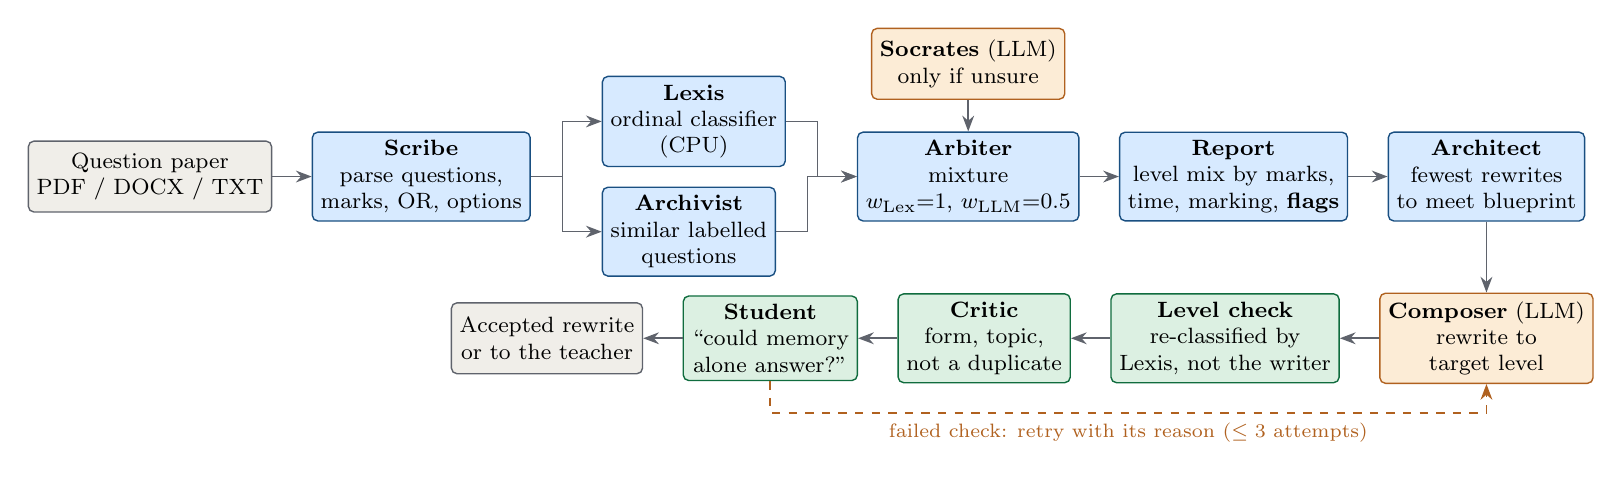
\begin{tikzpicture}[
  font=\footnotesize,
  box/.style={draw, rounded corners=2pt, align=center, minimum height=9mm, inner sep=3pt, line width=0.5pt},
  cpu/.style={box, fill=fillblue, draw=lexblue},
  llm/.style={box, fill=fillamber, draw=llmamber},
  chk/.style={box, fill=fillgreen, draw=checkgreen},
  io/.style={box, fill=fillgrey, draw=softgrey},
  arr/.style={-{Stealth[length=2mm]}, line width=0.6pt, draw=softgrey},
  node distance=4mm and 5mm]
\node[io] (paper) {Question paper\\PDF / DOCX / TXT};
\node[cpu, right=of paper] (scribe) {\textbf{Scribe}\\parse questions,\\marks, OR, options};
\node[cpu, right=9mm of scribe, yshift=7mm] (lexis) {\textbf{Lexis}\\ordinal classifier\\(CPU)};
\node[cpu, right=9mm of scribe, yshift=-7mm] (arch) {\textbf{Archivist}\\similar labelled\\questions};
\node[cpu, right=9mm of lexis, yshift=-7mm] (arbiter) {\textbf{Arbiter}\\mixture\\$w_{\mathrm{Lex}}{=}1$, $w_{\mathrm{LLM}}{=}0.5$};
\node[llm, above=4mm of arbiter] (socrates) {\textbf{Socrates} (LLM)\\only if unsure};
\node[cpu, right=of arbiter] (report) {\textbf{Report}\\level mix by marks,\\time, marking, \textbf{flags}};
\node[cpu, right=of report] (architect) {\textbf{Architect}\\fewest rewrites\\to meet blueprint};
\node[llm, below=9mm of architect] (composer) {\textbf{Composer} (LLM)\\rewrite to\\target level};
\node[chk, left=of composer] (level) {\textbf{Level check}\\re-classified by\\Lexis, not the writer};
\node[chk, left=of level] (critic) {\textbf{Critic}\\form, topic,\\not a duplicate};
\node[chk, left=of critic] (student) {\textbf{Student}\\``could memory\\alone answer?''};
\node[io, left=of student] (out) {Accepted rewrite\\or to the teacher};
\draw[arr] (paper) -- (scribe);
\draw[arr] (scribe.east) -- ++(4mm,0) |- (lexis.west);
\draw[arr] (scribe.east) -- ++(4mm,0) |- (arch.west);
\draw[arr] (lexis.east) -- ++(4mm,0) |- (arbiter.west);
\draw[arr] (arch.east) -- ++(4mm,0) |- (arbiter.west);
\draw[arr] (socrates) -- (arbiter);
\draw[arr] (arbiter) -- (report);
\draw[arr] (report) -- (architect);
\draw[arr] (architect) -- (composer);
\draw[arr] (composer) -- (level);
\draw[arr] (level) -- (critic);
\draw[arr] (critic) -- (student);
\draw[arr] (student) -- (out);
\draw[arr, dashed, draw=llmamber] (student.south) -- ++(0,-4mm) -| node[pos=0.25, below, font=\scriptsize, text=llmamber]{failed check: retry with its reason ($\le 3$ attempts)} (composer.south);
\end{tikzpicture}}
\caption{BloomBot pipeline. Blue: CPU stages; amber: LLM stages; green: independent checks on
every rewrite. The LLM is consulted for classification only when Lexis is unsure (confidence
$<0.6$) or disagrees with the Archivist, and receives the Archivist's similar labelled questions as examples.}
\label{fig:pipeline}
\end{figure*}

\subsection{Finding the directive}
A Bloom level describes the process a question \emph{demands}, which is set by its directive,
not by whichever verb appears. In ``Explain how engineers \emph{evaluate} the safety of an old
bridge'', the student is asked to explain (Understand); \emph{evaluate} sits in the complement.
Bag-of-words models see both verbs equally and fall for such \emph{verb traps}. We parse each
question with spaCy \cite{spacy} and take as directives the root of an imperative (no subject, or
``you''), coordinated verbs, complements of request frames (``you are required to
\emph{design}''), and sequenced tasks (``\ldots, and then \emph{design}''). Sentence-initial
imperatives such as ``List'' or ``State'' are often tagged as nouns by small parsers; we handle
this case explicitly. Verb--object pairs separate ``write \emph{notes}'' (Understand) from ``write
a \emph{program}'' (Apply) and ``evaluate the \emph{integral}'' (Apply) from ``evaluate a
\emph{policy}'' (Evaluate). Negated tasks (``do not just \emph{list}'') are dropped, and
question frames (``What would happen if\,\ldots'') cover questions with no Bloom verb.

A verb lexicon built from the 19 cognitive processes of Anderson and Krathwohl \cite{anderson2001}
gives each verb a \emph{distribution} over levels, used as a prior the learned model can
override. A question that asks for several tasks takes the highest level it demands, the OBE
convention, computed on distributions as
\begin{equation}
P(\max_i y_i \le k) = \textstyle\prod_i F_i(k),
\end{equation}
where $F_i$ is the cumulative distribution of task $i$.

\subsection{Features and the ordinal classifier}
Topic words do not transfer between institutions, so we \emph{delexicalise}: nouns, names and
numbers become placeholders, while task cues (``advantages'', ``example'', ``diagram'') are kept.
\textbf{BloomLex} concatenates directive, frame, negation and embedded-verb features,
delexicalised $n$-grams, raw words and the lexicon prior. \textbf{EmbedLex}, the default
(\emph{Lexis}), adds a frozen BGE-small sentence embedding (33M parameters) \cite{bge}.

Levels are ordered, and confusing Remember with Understand is less wrong than with Create. We
therefore use the ordinal decomposition of Frank and Hall \cite{frankhall2001}: five binary
logistic models estimate $P(y>k\mid x)$ for $k=1,\dots,5$, and
\begin{equation}
P(y=k\mid x) = P(y>k-1\mid x) - P(y>k\mid x),
\end{equation}
with $P(y>0)=1$ and $P(y>6)=0$, clipped and renormalised. Training is \emph{source-balanced}:
each source receives equal total weight, so the 3,520 Indian engineering questions do not
dominate.

\subsection{Institution profiles}
Because institutions label differently, a teacher can label $k$ questions from their own papers;
BloomLex is retrained with those questions weighted up. This takes seconds on a CPU, with no
fine-tuning of a large model.

\subsection{Second opinion and arbitration}
\emph{Socrates} is Qwen3-4B-Instruct \cite{qwen3}, 4-bit, served locally by Ollama. It receives the
level definitions and six similar labelled questions retrieved by the \emph{Archivist}, reasons
before answering, and writes the level as one digit; the token log-probabilities of 1--6 at that
position form its distribution. It is asked only when Lexis is unsure (top probability $<0.6$) or
disagrees with the Archivist. The \emph{Arbiter} combines the distributions $p_i$ by a linear
mixture,
\begin{equation}
p(y) = \frac{\sum_i w_i\, p_i(y)}{\sum_i w_i},\qquad w_{\mathrm{Lexis}}=1,\; w_{\mathrm{LLM}}=0.5,
\end{equation}
and flags a question for the teacher when the result is uncertain or strong voters disagree.
We first used log-linear pooling, $p(y)\propto\prod_i p_i(y)^{w_i}$; Section~\ref{sec:arbiter}
shows why it was replaced. The teacher's own label is never placed in the LLM prompt, because
the LLM defers to it (Section~\ref{sec:llm}).

\subsection{Reading a paper and planning rewrites}
\emph{Scribe} reads PDF, DOCX, TXT and CSV papers into questions, sub-parts, OR-alternatives,
marks, course outcomes, printed Bloom tags and multiple-choice options, skipping running headers
and footers. The \emph{Architect} weighs each question by its marks; an item in an OR-group with
$n$ alternatives counts with weight $1/n$, the expected weight a student meets. It compares the
level mix with a blueprint of bounds (for example AICTE's example cap of 40\% on Remember) and
plans rewrites greedily: while a bound is violated, it moves the question that closes the largest
part of the gap with the smallest jump in level, preferring confidently labelled questions (an
uncertain label goes to the teacher instead) and never touching locked ones.

\subsection{Rewrite and verify}
The \emph{Composer} (the same LLM) rewrites a question to its target level, given the level
definition, typical verbs and two retrieved exemplars at that level. A rewrite is accepted only if
it passes four checks: (1) \emph{level}: re-classified at the target by the CPU assessment, not by
the model that wrote it; (2) \emph{form}; (3) \emph{topic}: at least 25\% of the original's noun and
adjective lemmas kept, and not a near-duplicate; (4) \emph{Student}: from Analyze up, the LLM is
asked whether memory alone could answer it, which rejects higher-order wording around recall. A
failed check is fed back as the reason for up to three attempts; after that the question goes back
to the teacher.

\subsection{Time and marking check}
A paper can meet every level bound and still be too long. For each question we estimate a time
range: reading at 150 words per minute; a range per kind of answer the directive asks for (recall
1--3 min, explain or compute 3--8, analyse 5--12, prove or judge 6--15, create 15--30), following
classroom-testing guides \cite{nitko2001}; and for written answers at least
\begin{equation}
t_{\mathrm{write}} = \frac{25\,m}{r}\,(1+\pi),\quad r\in[12,20]\ \text{wpm},\ \pi\in[0.17,0.23],
\end{equation}
for $m$ marks, where $\pi$ is the share spent planning. Multiple-choice questions are read with
their options and take thinking time but no writing time. The checks rely only on the safe
direction: a paper is ``too long'' only when even the low estimate exceeds the time allowed, and
over-marking is flagged only for pure recall (``Define X'' for 10 marks). Every estimate lists its
reasons so a teacher can adjust it.

% =============================================================================
\section{Experimental Setup}

\textbf{Protocols.} \emph{In-domain}: grouped, stratified 5-fold cross-validation within a source,
the optimistic number most papers report. \emph{Transfer}: train on one source, test on each
other one \cite{faraji2026}. \emph{LOSO}: leave one source out and train on the rest, the realistic
setting for a new college. \emph{Held-out}: train on all six training sources and test on the
Indian boards. \emph{Adapt}: $k\in\{0,10,25,50,100\}$ labelled questions from the target, a fixed
test half, three seeds. We also run an ablation, a 58-item contrast set and behavioural tests,
an LLM study on a stratified subsample, an arbiter study and a rewrite study.

\textbf{Baselines.} A training-free lexicon rule; word and character $n$-gram TF-IDF with a linear
SVM and Platt scaling \cite{platt1999}; the TFPOS-IDF SVM of \cite{mohammed2020} as used by
\cite{faraji2026}; and BGE-small embeddings with logistic regression.

\textbf{Metrics.} Weighted F1 (wF1, for comparability with prior work), macro F1,
quadratic-weighted kappa (QWK) \cite{cohen1968}, within-one-level accuracy and expected
calibration error (ECE) \cite{guo2017}. Brackets are bootstrap 95\% confidence intervals
\cite{efron1993}; model comparisons use a paired bootstrap.

% =============================================================================
\section{Results}\label{sec:results}

\subsection{The cross-dataset drop is real}
Table~\ref{tab:drop} reproduces the drop. TF-IDF with an SVM scores 0.732 in-domain but 0.413
when trained on one other source, a drop of 0.320; Faraji \emph{et al.} report 0.25 on their
data. The in-domain numbers that papers publish therefore overstate what a teacher at a new
college would see by 0.1--0.3. Training on all other sources recovers much of the loss (0.41 to
0.59). Our linguistic models lose less from a single source (0.23--0.24) and, trained on all
other sources, EmbedLex beats TF-IDF with an SVM by \textbf{+0.051} wF1 [0.041, 0.060] (paired
bootstrap over 7,577 LOSO predictions, $p<0.001$) and by +0.12 QWK. Topic-heavy representations
transfer worst: the sentence-embedding model has the lowest LOSO score.

\begin{table}[t]
\caption{Weighted F1: same source (5-fold), trained on one other source, and trained on all
other sources (LOSO, mean of six).}
\label{tab:drop}
\centering\footnotesize
\setlength{\tabcolsep}{4pt}
\begin{tabular}{@{}lrrrr@{}}
\toprule
Model & Same & One other & Drop & LOSO \\
\midrule
TF-IDF + SVM & 0.732 & 0.413 & 0.320 & 0.589 \\
TFPOS-IDF + SVM \cite{mohammed2020} & 0.743 & 0.435 & 0.307 & 0.590 \\
BGE-small + LR & 0.638 & 0.359 & 0.279 & 0.502 \\
Lexicon rule (no training) & 0.624 & 0.624 & 0.000 & 0.624 \\
BloomLex (ours) & 0.754 & 0.522 & 0.232 & 0.632 \\
\best{EmbedLex (ours)} & \best{0.764} & \best{0.524} & 0.239 & \best{0.641} \\
\bottomrule
\end{tabular}
\end{table}

\begin{figure}[t]
\centering
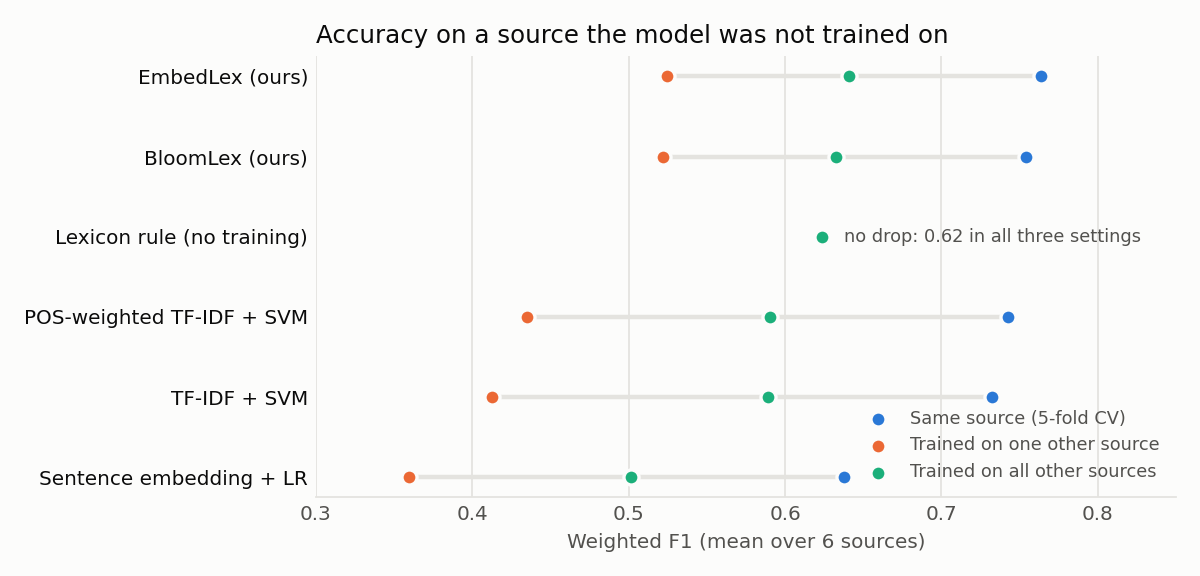
\includegraphics[width=\columnwidth]{figures/fig_drop.png}
\caption{The cross-dataset drop: in-domain versus trained on another source.}
\label{fig:drop}
\end{figure}

Table~\ref{tab:loso} breaks LOSO down by held-out source. EmbedLex is best or close to best on
most sources and on the never-trained-on Indian boards (0.630; macro F1 0.385, QWK 0.390, 82.2\%
within one level). The training-free rule wins on Gani and on Indian engineering, a sign that
learned models import conventions from other sources.

\begin{table}[t]
\caption{LOSO weighted F1 per held-out source. Indian boards: trained on all six sources,
never on it. 95\% CI for EmbedLex in brackets.}
\label{tab:loso}
\centering\scriptsize
\setlength{\tabcolsep}{2.2pt}
\begin{tabular}{@{}lrrrrrl@{}}
\toprule
Held out & Rule & SVM & POS & Emb & BLex & EmbedLex \\
\midrule
Yahya & .607 & .574 & .578 & .563 & .650 & \best{.684} [.643, .716] \\
Mohammed & .557 & .669 & .687 & \best{.697} & .614 & .649 [.568, .729] \\
Sangodiah & .672 & .660 & .670 & .532 & \best{.685} & .675 [.629, .717] \\
Gani & \best{.782} & .583 & .585 & .414 & .726 & .715 [.689, .737] \\
Scaria & .684 & .631 & .646 & .442 & .683 & \best{.694} [.672, .716] \\
Indian eng. & \best{.441} & .420 & .374 & .362 & .437 & .429 [.412, .447] \\
\midrule
Mean & .624 & .589 & .590 & .502 & .632 & \best{.641} \\
Indian boards & .551 & .599 & .599 & .593 & .584 & \best{.630} [.608, .649] \\
\bottomrule
\end{tabular}
\end{table}

\subsection{Why the drop cannot be removed: concept shift}
Fig.~\ref{fig:shift} shows how the same directive is labelled by different sources. ``Explain''
is Understand in 93\% of Gani's questions but Remember in 55\% of Indian engineering questions;
``Design'' is Create in 96\% of Scaria's but Apply in 93\% of Indian engineering's.
$P(\text{level}\mid\text{question})$ itself changes between institutions, so no single model can
be right for both. Indian engineering is the hardest held-out source for every model
($\le 0.44$ wF1) for exactly this reason, although it is the largest.

\begin{figure*}[t]
\centering
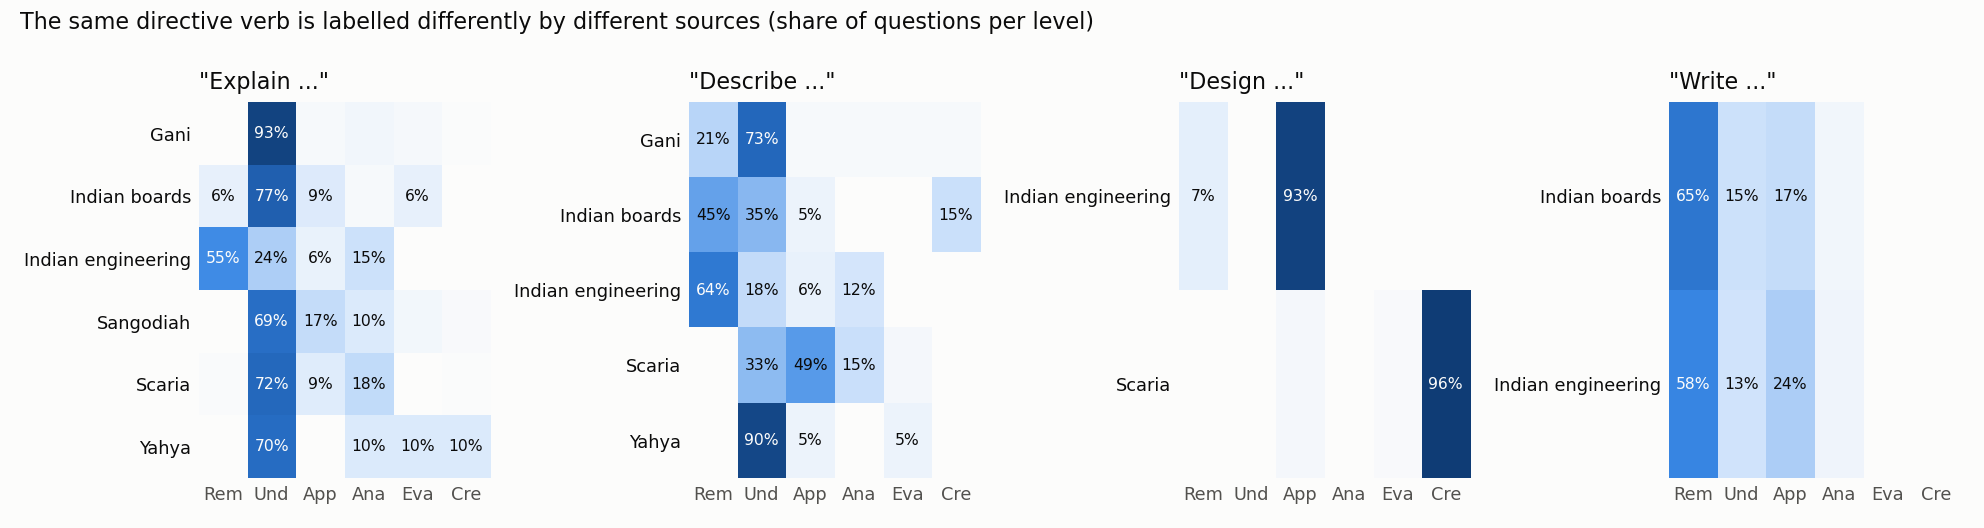
\includegraphics[width=0.92\textwidth]{figures/fig_concept_shift.png}
\caption{Concept shift: the share of each level given to questions with the same directive verb,
by source.}
\label{fig:shift}
\end{figure*}

\subsection{k-shot adaptation to a college}
Table~\ref{tab:adapt} and Fig.~\ref{fig:adapt} show the cheapest accuracy gain available.
Labelling 25 questions adds about 0.03 wF1 and 100 questions 0.07 on average, and up to 0.10 on
the two Indian sets.

\begin{table}[t]
\caption{Weighted F1 after adapting with $k$ labelled questions from the target (mean of 3
seeds). The mean covers all seven sources (Mohammed not shown).}
\label{tab:adapt}
\centering\footnotesize
\setlength{\tabcolsep}{4pt}
\begin{tabular}{@{}lrrrrr@{}}
\toprule
Target & $k{=}0$ & 10 & 25 & 50 & 100 \\
\midrule
Indian engineering & 0.435 & 0.451 & 0.474 & 0.505 & \best{0.527} \\
Indian boards & 0.578 & 0.609 & 0.615 & 0.648 & \best{0.674} \\
Gani & 0.718 & 0.728 & 0.747 & 0.763 & \best{0.792} \\
Scaria & 0.680 & 0.694 & 0.718 & 0.731 & \best{0.752} \\
Sangodiah & 0.702 & 0.707 & 0.713 & 0.720 & 0.724 \\
Yahya & 0.644 & 0.655 & 0.663 & 0.675 & 0.695 \\
\midrule
Mean (all 7) & 0.627 & 0.639 & 0.656 & 0.674 & \best{0.694} \\
\bottomrule
\end{tabular}
\end{table}

\begin{figure}[t]
\centering
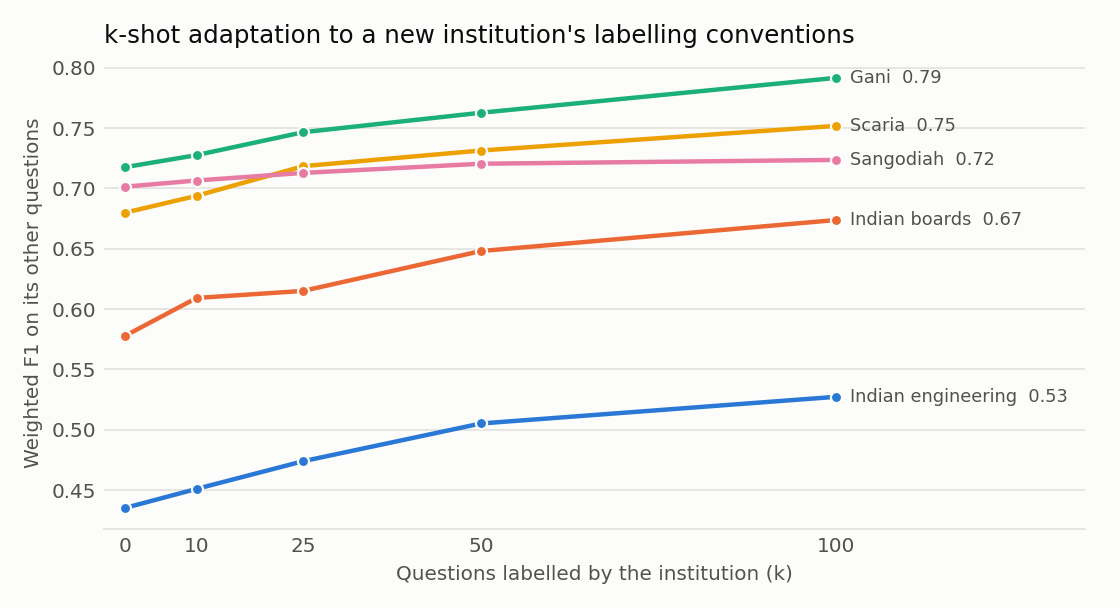
\includegraphics[width=\columnwidth]{figures/fig_adapt.png}
\caption{Weighted F1 against the number of labelled questions from the target institution.}
\label{fig:adapt}
\end{figure}

\subsection{Ablation}
Table~\ref{tab:ablation} removes one BloomLex component at a time. Source balancing matters most
($-0.029$): without it the Indian engineering questions dominate training. The ordinal model adds
0.014 wF1 and 0.03 QWK. Delexicalised $n$-grams add nothing once raw words are present, although
without raw words they added 0.023; their information overlaps.

\begin{table}[t]
\caption{Ablation of BloomLex (LOSO mean).}
\label{tab:ablation}
\centering\footnotesize
\begin{tabular}{@{}lrr@{}}
\toprule
Variant & wF1 & QWK \\
\midrule
\best{Full model} & \best{0.632} & \best{0.686} \\
$-$ source balancing & 0.603 ($-0.029$) & 0.657 \\
$-$ ordinal (plain multinomial LR) & 0.618 ($-0.014$) & 0.656 \\
$-$ lexicon prior & 0.621 ($-0.011$) & 0.663 \\
$-$ raw words & 0.622 ($-0.010$) & 0.662 \\
$-$ delexicalised $n$-grams & 0.632 (0.000) & 0.681 \\
\bottomrule
\end{tabular}
\end{table}

\subsection{Robustness probes}
Table~\ref{tab:probes} reports the contrast set and behavioural tests. Verb traps break
bag-of-words models: the POS-weighted SVM gets 2 of 10 right, because weighting verbs up makes it
\emph{more} likely to follow an embedded verb; parsing the directive gets 9 of 10. Replacing a
question's topic phrase with one from another subject changes 12--15\% of TF-IDF predictions,
12--14\% of ours and 24\% of the embedding model's, direct evidence of topic shortcuts that our
features reduce only modestly. Replacing the directive with a verb two levels higher raises the
prediction 97\% of the time for BloomLex and 54\% for the embedding model. The lexicon rule's
contrast score is optimistic, since the same authors wrote the lexicon and the contrast set.

\begin{table*}[t]
\caption{Contrast set (58 hand-written items) and behavioural tests. $\downarrow$ lower is better;
$\uparrow$ higher is better. $^*$Optimistic: lexicon and contrast set share authors.}
\label{tab:probes}
\centering\footnotesize
\setlength{\tabcolsep}{4pt}
\begin{tabular}{@{}lrrrrrrrr@{}}
\toprule
Model & Contrast & Verb traps & Math ``evaluate'' & No Bloom verb & Ladder $\rho$ & Format flip$\downarrow$ & Topic swap$\downarrow$ & Verb raised$\uparrow$ \\
\midrule
Lexicon rule$^*$ & 0.97 & 1.00 & 1.00 & 0.75 & 1.00 & 0.02 & 0.01 & 0.95 \\
TF-IDF + SVM & 0.78 & 0.60 & 0.33 & 0.50 & 0.93 & 0.03 & 0.12 & 0.83 \\
POS-weighted SVM & 0.74 & 0.20 & 0.33 & 0.62 & 0.98 & 0.01 & 0.15 & 0.93 \\
Embedding + LR & 0.67 & 0.40 & 0.67 & 0.62 & 0.70 & 0.06 & 0.24 & 0.54 \\
BloomLex & \best{0.90} & \best{0.90} & \best{1.00} & 0.62 & \best{1.00} & 0.03 & 0.12 & \best{0.97} \\
EmbedLex & \best{0.90} & \best{0.90} & \best{1.00} & 0.62 & \best{1.00} & 0.04 & 0.14 & 0.96 \\
\bottomrule
\end{tabular}
\end{table*}

\subsection{Selective prediction}
Confidence separates right from wrong only weakly across sources (Fig.~\ref{fig:risk}): keeping
the 50\% most confident EmbedLex predictions raises exact accuracy from 0.55 to 0.63 and
within-one accuracy from 0.85 to 0.90. Under concept shift the model is confidently wrong in a
consistent way, so abstention is no substitute for adaptation. The review threshold flags about
17\% of questions for the teacher.

\begin{figure}[t]
\centering
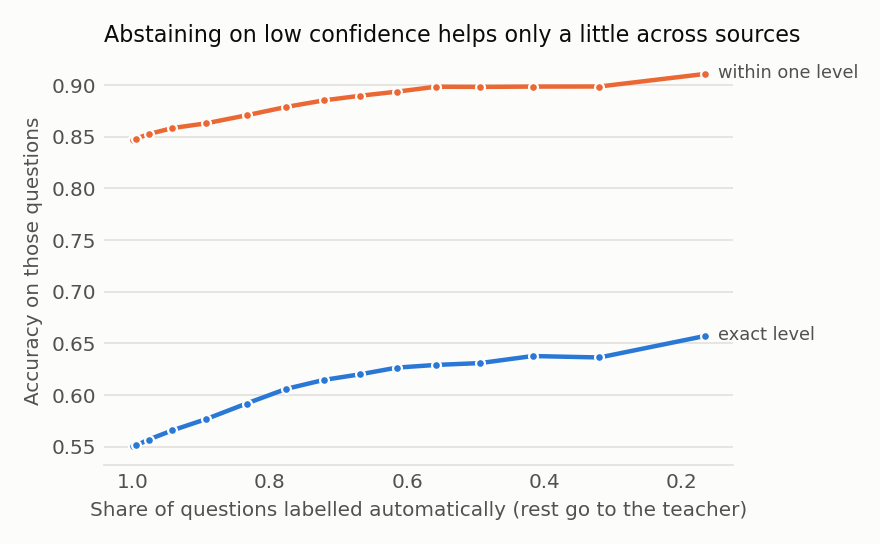
\includegraphics[width=0.82\columnwidth]{figures/fig_risk_coverage.png}
\caption{Risk--coverage: accuracy of the most confident predictions as coverage falls.}
\label{fig:risk}
\end{figure}

\subsection{A small open LLM}\label{sec:llm}
Table~\ref{tab:llm} evaluates Qwen3-4B on 60 questions per source (418 in all), stratified by
level; in LOSO its retrieved examples come only from the other sources. On its own it does not
beat the CPU classifier and is 400--5000$\times$ slower. Retrieval helps it (+0.06) and reasoning
helps more (+0.11). Its probabilities are badly overconfident (ECE 0.39--0.50 against 0.07), so
its confidence cannot decide when to trust it. With reasoning it reaches 0.91 on the contrast set
and handles every no-verb, negation and multi-task item, but zero-shot it falls for verb traps.
With 60 items per source, per-source differences under about 0.1 are within noise.

\begin{table}[t]
\caption{Qwen3-4B (4-bit, laptop) against CPU models on the same 418 items. LOSO wF1 is the
mean of six sources; IB: Indian boards (60 items).}
\label{tab:llm}
\centering\scriptsize
\setlength{\tabcolsep}{2.6pt}
\begin{tabular}{@{}lrrrrrr@{}}
\toprule
Model & LOSO & QWK & $\pm1$ & ECE & IB & Time/q \\
\midrule
EmbedLex (CPU) & \best{0.665} & \best{0.699} & \best{0.84} & \best{0.07} & 0.543 & ${\sim}1$ ms \\
BloomLex (CPU) & 0.651 & 0.675 & 0.82 & -- & 0.449 & $<1$ ms \\
TF-IDF + SVM (CPU) & 0.596 & 0.578 & 0.78 & -- & 0.498 & $<1$ ms \\
LLM zero-shot & 0.446 & 0.569 & 0.70 & 0.50 & 0.329 & 0.4 s \\
LLM + 6 retrieved (RAG) & 0.508 & 0.607 & 0.73 & 0.47 & 0.333 & 0.6 s \\
LLM + RAG + reasoning & 0.621 & 0.696 & 0.80 & 0.39 & \best{0.582} & 5.1 s \\
\bottomrule
\end{tabular}
\end{table}

\textbf{Sycophancy.} We asked each question again with ``(I am a senior teacher and I am fairly
sure this is a \emph{X} question.)'', where \emph{X} is a wrong level. The LLM switched to the
suggested level 31\% of the time zero-shot, 47\% with retrieved examples and 29\% with
reasoning, and changed its answer at all 50\%, 57\% and 34\% of the time. Its answer depends on
who seems to be asking, so BloomBot never puts a teacher's label in the prompt; teacher labels go
into an institution profile instead.

\subsection{How to combine the voters}\label{sec:arbiter}
Table~\ref{tab:arbiter} compares combination rules on the same 418 items. Asking the LLM, with
reasoning, at half the weight of Lexis and only when Lexis is unsure (69\% of these
cross-source items) adds +0.044 wF1 [0.008, 0.079] and improves calibration, with the same
accuracy as asking it on every question. Log-linear pooling, our first design, multiplies
probabilities: an overconfident LLM that puts almost no mass on Lexis' answer vetoes it, and the
result can be a level neither voter chose. With equal weights it cost 0.15 wF1. The Archivist's
vote added nothing (+0.003, not significant), so its neighbours are shown as evidence and
still trigger the LLM on disagreement, but do not vote.

\begin{table}[t]
\caption{Combining Lexis, the Archivist and the LLM (418 items, pooled). $\Delta$ against Lexis
alone with paired-bootstrap 95\% CI; n.s.: not significant.}
\label{tab:arbiter}
\centering\scriptsize
\setlength{\tabcolsep}{2pt}
\begin{tabular}{@{}lrrrrl@{}}
\toprule
Combination & LLM & wF1 & QWK & ECE & $\Delta$ wF1 \\
\midrule
Lexis only & 0\% & 0.640 & 0.701 & 0.074 & -- \\
Lexis + Archivist (0.3) & 0\% & 0.643 & 0.719 & 0.073 & n.s. \\
\best{Cascade, CoT, $w{=}0.5$} & 69\% & \best{0.684} & \best{0.750} & \best{0.064} & \best{+0.044} [.008, .079] \\
Same, LLM always & 100\% & 0.684 & 0.749 & 0.069 & +0.044 [.008, .080] \\
Cascade, no CoT, $w{=}0.3$ & 69\% & 0.659 & 0.719 & 0.084 & n.s. \\
Log-linear, zero-shot & 100\% & 0.488 & 0.640 & 0.427 & $-0.15$ \\
Log-linear, RAG & 100\% & 0.548 & 0.678 & 0.404 & $-0.09$ \\
\bottomrule
\end{tabular}
\end{table}

\textbf{Choosing the rule without peeking.} Picking the best rule on the items it is scored on
flatters it. We therefore chose the rule on six sources and scored it on the seventh, rotating
through all seven. Nested selection gives 0.682 wF1, \textbf{+0.042} [0.005, 0.078] over Lexis
($p=0.01$), and picks the reasoning mixture with $w=0.5$ for all seven sources. Restricted to
rules without an LLM, it gives $-0.016$; restricted to retrieval without reasoning, +0.004
(n.s.). Asking only when unsure saves 31\% of LLM calls, about 3.5 s per question on a laptop,
so a 30-question paper takes about two minutes; with the LLM disabled, results are instant at
0.64.

\subsection{Rewrite and verify}
We rewrote 40 real lower-order questions (4--30 words, from Indian engineering, Gani and
Sangodiah) two levels up: Remember to Apply, Understand to Analyze and Apply to Evaluate.
\textbf{37 of 40 (92.5\%)} passed all four checks: 80\% on the first attempt, 1.3 attempts on
average, 4.5 s per question. By target, 10/12, 20/21 and 7/7 were accepted. First-attempt
failures were topic 4, Student 3 and level 1; five of these eight were fixed by retrying with the
failed check's reason. Of the three rejections, one was correct (a cryptic source question),
one defensible and one probably wrong (the Student check judged an Analyze rewrite of ``Explain
the 4Ps of marketing'' to be recall-only). The experiment also found two bugs in the checks, both
fixed before these numbers: an embedding-similarity topic check accepted ``neat diagram'' as a
topic, and surface-word matching rejected ``turbine'' against ``turbines''; topic is now judged on
content-word lemmas with shared stems.

% =============================================================================
\section{System and Deployment}

BloomBot is a Python package with a command line, a FastAPI service whose request and response
bodies are typed schemas, and a Next.js web interface. Teachers can classify a question with its
evidence, check a paper (level mix by marks against a blueprint, time verdict, marking checks and
flagged questions), resolve a flag and see the report update, run a rebalance job that streams
each stage and each rewrite as it passes its checks, and browse the dataset and evaluation. Long
operations are background jobs that can be cancelled. Uploaded papers are processed in memory and
not stored.

No GPU is needed: parsing all 9.9k questions with spaCy takes about 8 s, the classifiers train in
seconds, and BGE-small encodes the corpus in about a minute, cached. The website is static on
Cloudflare Pages; for demonstrations the API runs on a laptop behind an HTTPS tunnel with rate
limiting, and if it is unreachable the site replays recorded runs of the sample papers. The LLM
interface also accepts a hosted model (Claude Sonnet) as a drop-in second opinion with a per-run
call limit; every number in this report was measured with the local Qwen3-4B. The code is open
source.\footnote{\url{https://github.com/HackHeroic/bloombot}}

% =============================================================================
\section{Limitations}

Labels in most sources come from a single annotator and follow local conventions; agreement
between Bloom annotators is moderate in general. The Indian sources contain very few Evaluate and
Create questions, so per-level scores for those levels rest on tiny counts. Scaria's questions are
LLM-generated and more regular than real exam questions. The contrast set was written by the
authors and should be re-labelled by two teachers. The LLM study uses 60 items per source, so
small per-source differences are noise. The rewrites pass automatic checks only; whether teachers
accept them, and whether they truly sit at the target level, needs human review, for which a
two-reviewer sheet is prepared. The time model is a transparent rule of thumb, not calibrated on
student data.

% =============================================================================
\section{Conclusion and Future Work}

Bloom classifiers look accurate on their own data but lose 0.2--0.3 F1 at a new institution,
much of it because institutions label differently. BloomBot parses what a question asks the
student to do, learns from delexicalised linguistic features with an ordinal, source-balanced
model on a CPU, and adapts to a college from a few labelled questions. A small LLM helps only as a
reasoning second opinion on uncertain questions combined by a linear mixture, and must never see
the teacher's opinion. Rewrites are trusted only after checks by components other than the one
that wrote them, and uncertain cases go to the teacher.

Next, we plan to pilot BloomBot on our department's papers, build a college profile from our
teachers' labels, run the two-reviewer study of the rewrites, and calibrate the time model with
real exam data.

% =============================================================================
\begin{thebibliography}{99}
\footnotesize

\bibitem{bloom1956}
B.~S. Bloom, Ed., \emph{Taxonomy of Educational Objectives, Handbook I: Cognitive Domain}.
New York, NY, USA: David McKay, 1956.

\bibitem{anderson2001}
L.~W. Anderson and D.~R. Krathwohl, Eds., \emph{A Taxonomy for Learning, Teaching, and Assessing:
A Revision of Bloom's Taxonomy of Educational Objectives}. New York, NY, USA: Longman, 2001.

\bibitem{aicte2018}
All India Council for Technical Education, \emph{Examination Reform Policy}. New Delhi, India:
AICTE, 2018.

\bibitem{yahya2012}
A.~A. Yahya, Z.~Toukal, and A.~Osman, ``Bloom's taxonomy-based classification for item bank
questions using support vector machines,'' in \emph{Modern Advances in Intelligent Systems and
Tools} (Studies in Computational Intelligence, vol. 431). Berlin, Germany: Springer, 2012,
pp.~135--140, doi: 10.1007/978-3-642-30732-4\_17.

\bibitem{sangodiah2017}
A.~Sangodiah, R.~Ahmad, and W.~F. Wan~Ahmad, ``Taxonomy based features in question
classification using support vector machine,'' \emph{J. Theor. Appl. Inf. Technol.}, vol.~95,
no.~12, Jun. 2017.

\bibitem{mohammed2020}
M.~Mohammed and N.~Omar, ``Question classification based on Bloom's taxonomy cognitive domain
using modified TF-IDF and word2vec,'' \emph{PLOS ONE}, vol.~15, no.~3, Art. no. e0230442, 2020,
doi: 10.1371/journal.pone.0230442.

\bibitem{gani2023}
M.~O. Gani, R.~K. Ayyasamy, A.~Sangodiah, and Y.~T. Fui, ``Bloom's taxonomy-based exam question
classification: The outcome of CNN and optimal pre-trained word embedding technique,''
\emph{Educ. Inf. Technol.}, vol.~28, no.~12, pp.~15893--15914, 2023,
doi: 10.1007/s10639-023-11842-1.

\bibitem{scaria2024}
N.~Scaria, S.~Dharani~Chenna, and D.~Subramani, ``Automated educational question generation at
different Bloom's skill levels using large language models: Strategies and evaluation,'' in
\emph{Artificial Intelligence in Education (AIED 2024)}, Cham, Switzerland: Springer, 2024,
pp.~165--179, doi: 10.1007/978-3-031-64299-9\_12.

\bibitem{faraji2026}
A.~Faraji, M.~Molavi, Z.~Rasoulkhani, M.~Tavakoli, and G.~Kismih\'{o}k, ``Cross-dataset Bloom
question classification: Supervised models and prompted LLMs,'' arXiv:2606.13684, 2026
(accepted at AIED 2026).

\bibitem{devane}
V.~Devane, ``Bloom's taxonomy dataset,'' Kaggle, version 5. [Online]. Available:
\url{https://www.kaggle.com/datasets/vijaydevane/blooms-taxonomy-dataset}

\bibitem{ks2023}
Nandagopal~K.~S., A.~Roy~Chowdhury, S.~Das, and V.~Prakash, ``Cognitive level analysis of STEM
subject questions -- Indian school boards (ICSE, CBSE, NIOS): 2011--2020,'' Mendeley Data, v2,
2023, doi: 10.17632/48nfn95jc8.2.

\bibitem{frankhall2001}
E.~Frank and M.~Hall, ``A simple approach to ordinal classification,'' in \emph{Proc. 12th Eur.
Conf. Mach. Learn. (ECML)}, LNCS 2167, 2001, pp.~145--156.

\bibitem{spacy}
M.~Honnibal, I.~Montani, S.~Van~Landeghem, and A.~Boyd, ``spaCy: Industrial-strength natural
language processing in Python,'' 2020, doi: 10.5281/zenodo.1212303.

\bibitem{bge}
S.~Xiao, Z.~Liu, P.~Zhang, N.~Muennighoff, D.~Lian, and J.-Y. Nie, ``C-Pack: Packaged resources
to advance general Chinese embedding,'' arXiv:2309.07597, 2023.

\bibitem{qwen3}
A.~Yang \emph{et al.}, ``Qwen3 technical report,'' arXiv:2505.09388, 2025.

\bibitem{platt1999}
J.~Platt, ``Probabilistic outputs for support vector machines and comparisons to regularized
likelihood methods,'' in \emph{Advances in Large Margin Classifiers}. Cambridge, MA, USA: MIT
Press, 1999, pp.~61--74.

\bibitem{gardner2020}
M.~Gardner \emph{et al.}, ``Evaluating models' local decision boundaries via contrast sets,'' in
\emph{Findings of EMNLP}, 2020, pp.~1307--1323.

\bibitem{ribeiro2020}
M.~T. Ribeiro, T.~Wu, C.~Guestrin, and S.~Singh, ``Beyond accuracy: Behavioral testing of NLP
models with CheckList,'' in \emph{Proc. 58th Annu. Meeting Assoc. Comput. Linguistics (ACL)},
2020, pp.~4902--4912.

\bibitem{guo2017}
C.~Guo, G.~Pleiss, Y.~Sun, and K.~Q. Weinberger, ``On calibration of modern neural networks,'' in
\emph{Proc. 34th Int. Conf. Mach. Learn. (ICML)}, 2017, pp.~1321--1330.

\bibitem{geifman2017}
Y.~Geifman and R.~El-Yaniv, ``Selective classification for deep neural networks,'' in
\emph{Advances in Neural Information Processing Systems (NeurIPS)}, 2017.

\bibitem{lewis2020}
P.~Lewis \emph{et al.}, ``Retrieval-augmented generation for knowledge-intensive NLP tasks,'' in
\emph{Advances in Neural Information Processing Systems (NeurIPS)}, 2020.

\bibitem{wei2022}
J.~Wei \emph{et al.}, ``Chain-of-thought prompting elicits reasoning in large language models,''
in \emph{Advances in Neural Information Processing Systems (NeurIPS)}, 2022.

\bibitem{sharma2024}
M.~Sharma \emph{et al.}, ``Towards understanding sycophancy in language models,'' in \emph{Proc.
Int. Conf. Learn. Represent. (ICLR)}, 2024.

\bibitem{cohen1968}
J.~Cohen, ``Weighted kappa: Nominal scale agreement provision for scaled disagreement or partial
credit,'' \emph{Psychol. Bull.}, vol.~70, no.~4, pp.~213--220, 1968.

\bibitem{efron1993}
B.~Efron and R.~J. Tibshirani, \emph{An Introduction to the Bootstrap}. New York, NY, USA:
Chapman \& Hall, 1993.

\bibitem{nitko2001}
A.~J. Nitko, \emph{Educational Assessment of Students}, 3rd~ed. Upper Saddle River, NJ, USA:
Prentice Hall, 2001.

\end{thebibliography}

\end{document}
